\documentclass[11pt]{article}
\usepackage{color}
\usepackage{graphicx}
\usepackage{amsmath,amsthm,amssymb,multirow,paralist}
\usepackage[margin=0.8in]{geometry}
\usepackage{hyperref}
\usepackage{tikz}
\usetikzlibrary{arrows.meta, positioning}
\usepackage{changepage}

\begin{document}

\begin{center}
{\Large \textbf{COM S 5730 Homework 3}}\\

\linethickness{1mm}\line(1,0){498}

\begin{enumerate}
\item Please put required code files and report into a
compressed file ``HW3\_FirstName\_LastName.zip''
\item Unlimited number of submissions are
allowed on Canvas and the latest one will be graded.
\item Due: \textbf{Tuesday Oct. 15, 2024 at 11:59pm.}
\item {\color{red} No later submission is accepted.}
\item Please read and follow submission instructions. No exception
will be made to accommodate incorrectly submitted files/reports.
\item All students are required to typeset their reports using
latex. Overleaf
(\url{https://www.overleaf.com/learn/latex/Tutorials}) can be a
good start.
\end{enumerate}

\linethickness{1mm}\line(1,0){498}

\end{center}

%%%%%%%%%%%%%%%%%%%%%%%%%%%%%%%%%%%%%%%%%%%%%%%%%%%%%%%%%%%%%%%%%%%%%%%%%%%%%%%

%%%%%%%%%%%%%%%%%%%%%%%%%%%%%%%%%%%%%%%%%%%%%%%%%%%%%%%%%%%%%%%%%%%%%%%%%%%%%%%


\begin{enumerate}

\item (15 points) You are provided with a training set of
examples (see Figure~\ref{fig:tree}). Which feature will you pick
first to split the data as per the ID3 decision tree learning
algorithm? Show all your work: compute the information gain for
all the four attributes and pick the best one.

\begin{figure*}[ht]\label{fig:tree}
\begin{center}
    \includegraphics[width=0.6\textwidth]{tree.jpg}
    \caption{Table with training examples. Each row corresponds
    to a single training example. There are four features,
    namely, outlook, temperature, humidity, and wind.
    ``PlayTennis'' is the class label.}
\end{center}
\end{figure*}

\textbf{Answer}

In order to compute the Information Gain of each feature, we need to first compute the entropy of the dataset:

\[
H(S) = - \sum_{i=1}^K P(S=y_i) \log_2 P(S=y_i)
\]

\textbf{PlayTenis (PT) - Entropy}

\[
\begin{aligned}
H(PT)&= -P(PT=Yes) \log_2 P(PT=Yes)-P(PT=No) \log_2 P(PT=No)\\[5pt]
&= -\frac{9}{14}\log_2\frac{9}{14}-\frac{5}{14}\log_2\frac{5}{14}\\[5pt]
&= .4097 + .5305\\[5pt]
&= .9402
\end{aligned}
\]\\

Now, let's calculate the feature entropy and calculate the Information Gain for them.\\

\textbf{Outlook (O) - Entropy}

\begin{tabular}{l|l|l}
    \textbf{Outlook = Rain} & \textbf{Outlook = Overcast} & \textbf{Outlook = Sunny} \\
    \hline
    $P(Outlook = Rain) = \frac{5}{14}$ & $P(Outlook = Overcast) = \frac{4}{14}$ & $P(Outlook = Sunny) = \frac{5}{14}$ \\
    $Yes: 3$ & $Yes: 4$ & $Yes: 2$ \\
    $No: 2$ & $No: 0$ & $No: 3$ \\
\end{tabular}\\\\

\textbf{Outlook = Rain}

\[
\begin{aligned}
H(O_R)&= -P(O_R=True) \log_2 P(O_R=True)-P(O_R=False) \log_2 P(O_R=False)\\[5pt]
&= -\frac{3}{5}\log_2\frac{3}{5}-\frac{2}{5}\log_2\frac{2}{5}\\[5pt]
&= .4421 + .5288\\[5pt]
&= .9709
\end{aligned}
\]

\textbf{Outlook = Sunny}

\[
\begin{aligned}
H(O_S)&= -P(O_S=True) \log_2 P(O_S=True)-P(O_S=False) \log_2 P(O_S=False)\\[5pt]
&= -\frac{2}{5}\log_2\frac{2}{5}-\frac{3}{5}\log_2\frac{3}{5}\\[5pt]
&= .5288 + .4421\\[5pt]
&= .9709
\end{aligned}
\]

\textbf{Outlook = Overcast}

\[
\begin{aligned}
H(O_O)&= -P(O_O=True) \log_2 P(O_O=True)-P(O_O=False) \log_2 P(O_O=False)\\[5pt]
&= -\frac{4}{4}\log_2\frac{4}{4}-\frac{0}{4}\log_2\frac{0}{4}\\[5pt]
&= 0
\end{aligned}
\]

\textbf{Outlook - Weighted Entropy}

\[
\begin{aligned}
H(O)&= P(O_R)H(O_R)+P(O_S)H(O_S)+P(O_O)H(O_O)\\[5pt]
&= (\frac{5}{14})(.9709)+(\frac{5}{14})(.9709)+(\frac{4}{14})(0)\\[5pt]
&= .6935
\end{aligned}
\]

\textbf{Outlook - Information Gain (IG)}

\[
\begin{aligned}
IG(O)&= H(PT) - H(O)\\[5pt]
&= .9402 - .6935\\[5pt]
&= .2467
\end{aligned}
\]

\textbf{Temperature (T) - Entropy}

\begin{tabular}{l|l|l}
    \textbf{Temperature = Cool} & \textbf{Temperature = Mild} & \textbf{Outlook = Hot} \\
    \hline
    $P(Temperature = Cool) = \frac{4}{14}$ & $P(Temperature = Mild) = \frac{6}{14}$ & $P(Temperature = Hot) = \frac{4}{14}$ \\
    $Yes: 3$ & $Yes: 4$ & $Yes: 2$ \\
    $No: 1$ & $No: 2$ & $No: 2$ \\
\end{tabular}\\\\

\textbf{Temperature = Cool}

\[
\begin{aligned}
H(T_C)&= -P(T_C=True) \log_2 P(T_C=True)-P(T_C=False) \log_2 P(T_C=False)\\[5pt]
&= -\frac{3}{4}\log_2\frac{3}{4}-\frac{1}{4}\log_2\frac{1}{4}\\[5pt]
&= .3113 + .5\\[5pt]
&= .8113
\end{aligned}
\]

\textbf{Temperature = Mild}

\[
\begin{aligned}
H(T_M)&= -P(T_M=True) \log_2 P(T_M=True)-P(T_M=False) \log_2 P(T_M=False)\\[5pt]
&= -\frac{4}{6}\log_2\frac{4}{6}-\frac{2}{6}\log_2\frac{2}{6}\\[5pt]
&= .3899 + .5283\\[5pt]
&= .9182
\end{aligned}
\]

\textbf{Temperature = Hot}

\[
\begin{aligned}
H(T_H)&= -P(T_H=True) \log_2 P(T_H=True)-P(T_H=False) \log_2 P(T_H=False)\\[5pt]
&= -\frac{2}{4}\log_2\frac{2}{4}-\frac{2}{4}\log_2\frac{2}{4}\\[5pt]
&= .5 + .5\\[5pt]
&= 1
\end{aligned}
\]

\textbf{Temperature - Weighted Entropy}

\[
\begin{aligned}
H(T)&= P(T_C)H(T_C)+P(T_M)H(T_M)+P(T_H)H(T_H)\\[5pt]
&= (\frac{4}{14})(.8113)+(\frac{6}{14})(.9182)+(\frac{4}{14})(1)\\[5pt]
&= .9109
\end{aligned}
\]

\textbf{Temperature - Information Gain (IG)}

\[
\begin{aligned}
IG(T)&= H(PT) - H(T)\\[5pt]
&= .9402 - .9109\\[5pt]
&= .0293
\end{aligned}
\]

\textbf{Humidity (H) - Entropy}

\begin{tabular}{l|l|l}
    \textbf{Humidity = Normal} & \textbf{Humidity = High} \\
    \hline
    $P(Humidity = Normal) = \frac{7}{14}$ & $P(Humidity = High) = \frac{7}{14}$ \\
    $Yes: 6$ & $Yes: 3$ \\
    $No: 1$ & $No: 4$\\
\end{tabular}\\\\

\textbf{Humidity = Normal}

\[
\begin{aligned}
H(H_N)&= -P(H_N=True) \log_2 P(H_N=True)-P(H_N=False) \log_2 P(H_N=False)\\[5pt]
&= -\frac{6}{7}\log_2\frac{6}{7}-\frac{1}{7}\log_2\frac{1}{7}\\[5pt]
&= .1907 + .4011\\[5pt]
&= .5918
\end{aligned}
\]

\textbf{Humidity = High}

\[
\begin{aligned}
H(H_H)&= -P(H_H=True) \log_2 P(H_H=True)-P(H_H=False) \log_2 P(H_H=False)\\[5pt]
&= -\frac{3}{7}\log_2\frac{3}{7}-\frac{4}{7}\log_2\frac{4}{7}\\[5pt]
&= .5239 + .4614\\[5pt]
&= .9853
\end{aligned}
\]

\textbf{Humidity - Weighted Entropy}

\[
\begin{aligned}
H(H)&= P(H_N)H(H_N)+P(H_H)H(H_H)\\[5pt]
&= (\frac{7}{14})(.5918)+(\frac{7}{14})(.9853)\\[5pt]
&= .7885
\end{aligned}
\]

\textbf{Humidity - Information Gain (IG)}

\[
\begin{aligned}
IG(H)&= H(PT) - H(H)\\[5pt]
&= .9402 - .7885\\[5pt]
&= .1517
\end{aligned}
\]

\textbf{Wind (W) - Entropy}

\begin{tabular}{l|l|l}
    \textbf{Wind = Weak} & \textbf{Wind = Strong} \\
    \hline
    $P(Wind = Weak) = \frac{8}{14}$ & $P(Wind = Strong) = \frac{6}{14}$ \\
    $Yes: 6$ & $Yes: 3$ \\
    $No: 2$ & $No: 3$\\
\end{tabular}\\\\

\textbf{Wind = Weak}

\[
\begin{aligned}
H(W_W)&= -P(W_W=True) \log_2 P(W_W=True)-P(W_W=False) \log_2 P(W_W=False)\\[5pt]
&= -\frac{6}{8}\log_2\frac{6}{8}-\frac{2}{8}\log_2\frac{2}{8}\\[5pt]
&= .3113 + .5\\[5pt]
&= .8113
\end{aligned}
\]

\textbf{Wind = Strong}

\[
\begin{aligned}
H(W_S)&= -P(W_S=True) \log_2 P(W_S=True)-P(W_S=False) \log_2 P(W_S=False)\\[5pt]
&= -\frac{3}{6}\log_2\frac{3}{6}-\frac{3}{6}\log_2\frac{3}{6}\\[5pt]
&= .5 + .5\\[5pt]
&= 1
\end{aligned}
\]

\textbf{Wind - Weighted Entropy}

\[
\begin{aligned}
H(W)&= P(W_W)H(W_W)+P(W_S)H(W_S)\\[5pt]
&= (\frac{8}{14})(.8113)+(\frac{6}{14})(1)\\[5pt]
&= .8922
\end{aligned}
\]

\textbf{Wind - Information Gain (IG)}

\[
\begin{aligned}
IG(W)&= H(PT) - H(W)\\[5pt]
&= .9402 - .8922\\[5pt]
&= .0480
\end{aligned}
\]

\textbf{Final Decision}

$IG(Outlook) = .247$\\
$IG(Humidity) = .152$\\
$IG(Wind) = .048$\\
$IG(Temperature) = .029$\\

I'll pick the \textbf{Outlook} feature first to split the data as per ID3 decision tree learning algorithm because it has the highest Information Gain among the given features, which is .247.

\item (15 points) We know that we can convert any decision tree
into a set of if-then rules, where there is one rule per leaf
node. Suppose you are given a set of rules $R = \{r_1, r_2,
\dots, r_k\}$, where $r_i$ corresponds to the $i^{th}$ rule.
{\color{red} These rules are valid and complete, which means
there is no conflicting rules. You can always obtain a prediction
based on these rules.} Is it possible to convert the rule set $R$
into an equivalent decision tree? Explain your construction or
give a counterexample.

\textbf{Answer}

Given the set of rules are valid and complete, it's always possible to convert the set R into an equivalent decision tree. The construction involves using the conditions of each rule as branches from the root node to the leaf node, ensuring that the decision tree provides the same output as the given set of rules.

Suppose we have the following rules:

\textbf{Rule 1:} If $A=1$ and $B=2$, then $Class=0$.\\
\textbf{Rule 2:} If $A=1$ and $B=3$, then $Class=1$.\\
\textbf{Rule 3:} If $A=2$, then $Class=2$.

Then, we have the following tree:

\begin{figure}[ht]
    \centering
    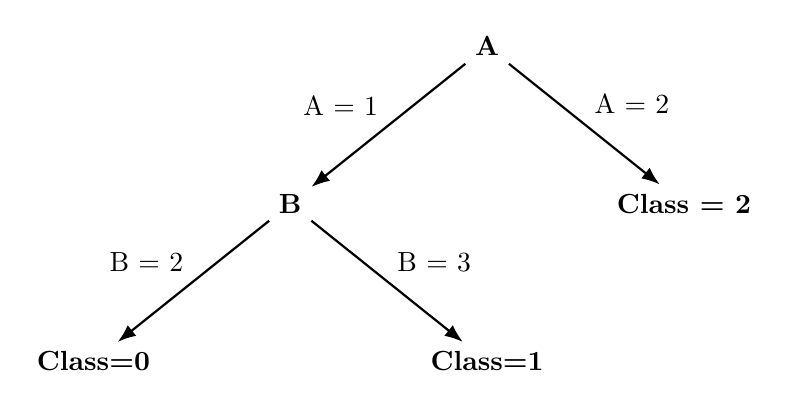
\begin{tikzpicture}[
        level distance=2cm,
        sibling distance=5cm,
        edge from parent/.style={draw, -{Latex}, thick}
    ]

    % Root node (A)
    \node {\textbf{A}}
        % Left child of A (A = 1)
        child {
            node {\textbf{B}} 
            child {
                node {\textbf{Class=0}}
                edge from parent node[above left] {B = 2}
                }
            child {
                node {\textbf{Class=1}}
                edge from parent node[above right] {B = 3}
                }
            edge from parent node[above left] {A = 1}}
        % Right child of A (A = 2)
        child {
            node {\textbf{Class = 2}}
            edge from parent node[above right] {A = 2}
        };

    \end{tikzpicture}
    \caption{Decision Tree Representation}
\end{figure}


\item (20 points) Suppose $\boldsymbol x = [x_1, x_2, \dots,
x_d]$ and $\boldsymbol z = [z_1, z_2, \dots, z_d]$ be two points in
a high-dimensional space (i.e., $d$ is very large).

\begin{enumerate}
    \item (10 points) Try to prove the following, where the
    right-hand side quantity represent the standard Euclidean
    distance.
    \begin{align*}
        \left(\frac{1}{\sqrt{d}}\sum_{i=1}^d x_i - \frac{1}{\sqrt{d}} \sum_{i=1}^d z_i \right)^2 \le
        \sum_{i=1}^d \left(x_i - z_i\right)^2
    \end{align*}

    \textbf{Hint: } Use Jensen’s inequality – If $X$ is a random
    variable and $f$ is a convex function, then $f(E[X]) \le
    E[f(X)]$.\\

    \textbf{Answer}

\begin{itemize}
    \item If we denote: 
    \[y_i=x_i-z_i\]

    \item The inequality becomes:

    \[(\frac{1}{\sqrt{d}}\sum_{i=1}^d y_i)^2 \leq \sum_{i=1}^d y_i^2\] \textbf{Note}: $f(x) = x^2$, which is a \textbf{convex function}.

    \item Consider $y_i$ as samples of a random variable Y, with \textbf{equal probability}. That means the probability associated to each $y_i$ is $p_i = \frac{1}{d}$

    \begin{itemize}
        \item Expected value of Y:

        \[
        E[Y] = \sum_{i=1}^d p_iy_i = \frac{1}{d} \sum_{i=1}^d y_i
        \]
        \item Expected value of $Y^2$:

        \[
        E[Y^2] = \sum_{i=1}^d p_iy_i^2 = \frac{1}{d} \sum_{i=1}^d y_i^2
        \]
    \end{itemize}

    \item Jensen's Inequality with $f(x) = x^2$ function.
    \[(E[Y])^2 \le E[Y^2]\]
        
    \item Substitute the expected values.
    \begin{align*}
    \left(\frac{1}{d} \sum_{i=1}^d y_i\right)^2 \le \frac{1}{d} \sum_{i=1}^d y_i^2
    \end{align*}

    \item Multiply both sides by d, we get:
    \begin{align*}
    \left(\frac{1}{\sqrt{d}}\sum_{i=1}^d y_i\right)^2 \leq \sum_{i=1}^d y_i^2
    \end{align*}

    \item Substitute $y_i$ back to $x_i - z_i$.
    \begin{align*}
    \left(\frac{1}{\sqrt{d}}\sum_{i=1}^d (x_i-z_i)\right)^2 \leq \sum_{i=1}^d (x_i-z_i)^2
    \end{align*}

    \begin{align*}
    \left(\frac{1}{\sqrt{d}}\sum_{i=1}^d x_i-\frac{1}{\sqrt{d}}\sum_{i=1}^d z_i\right)^2 
        \leq \sum_{i=1}^d (x_i-z_i)^2
    \end{align*}

This brings us back to the original inequality, thereby proving that the inequality holds for the given points $x$ and $z$ in high-dimensional space.\\

\end{itemize}
    
    \item (10 points) We know that the computation of nearest
    neighbors is very expensive in the high-dimensional space.
    Discuss how we can make use of the above property to make the
    nearest neighbors computation efficient?

\textbf{Answer}

By using Jensen's inequality, we can quickly estimate a lower bound on the distance between points. This allows us to skip over points that are obviously too far away, which means we don't have to calculate the full distance for every single point. By reducing these unnecessary calculations, we make the nearest neighbor search much faster, especially in high-dimensional spaces.

\end{enumerate}

\item (50 points) \textbf{Car Evaluation}: You will
build a Car Evaluation classifier. This classifier will be
used to classify the condition of a car.

The data: car\_evaluation.csv. This is the data
consisting of car evaluations. 

\begin{enumerate}
\item (20 points) Implement the ID3 decision tree learning
algorithm that we discussed in the class. The key step in the
decision tree learning is choosing the next feature to split on.
Implement the information gain heuristic for selecting the next
feature. Please see lecture notes or
\url{https://en.wikipedia.org/wiki/ID3_algorithm} for more
details.

\item (20 points) Implement the decision tree pruning algorithm
discussed in the class (via validation data).

\item (10 points) Compute the accuracy of decision tree and
pruned decision tree on validation examples and testing examples.
List your observations by comparing the performance of decision
tree with and without pruning.

\begin{adjustwidth}{2cm}{2cm}
\begin{verbatim}
==========================================================
Validate accuracy on tree without pruning ========> 0.8881
Validate accuracy on tree with pruning ===========> 0.6895
Test accuracy on tree without pruning ============> 0.8757
Test accuracy on tree with pruning ===============> 0.6908
Tree size without pruning ========================>    288
Tree size with pruning ===========================>      4
Tree depth without pruning =======================>      7
Tree depth with pruning ==========================>      2
==========================================================
\end{verbatim}
\end{adjustwidth}
\end{enumerate}

\textbf{Accuracy Comparison}
    
    Both validation and test accuracy decreased after pruning (validation: 0.8881 to 0.6895, test: 0.8757 to 0.6908). This suggests that the pruned tree may be under-fitting compared to the non-pruned version, as it has lost predictive power on both datasets.

\textbf{Tree Complexity}

    The pruned tree has significantly reduced size (from 288 nodes to 4 nodes) and depth (from 7 to 2). This reduction in complexity makes the model simpler, which resulted in the under-fitting observed in this experiment.

\textbf{Generalization vs. Fit}

    Although pruning generally aims to reduce over-fitting and improve generalization, in this case, it appears that pruning caused under-fitting, resulting in lower performance on both the validation and test datasets.
    

\end{enumerate}

\end{document}
